%----------------------------------------------------------------------
% Problem 3

\begingroup
\allowdisplaybreaks

\newpage
\section*{Problem 3}

\begin{figure}[h]
	\centering
	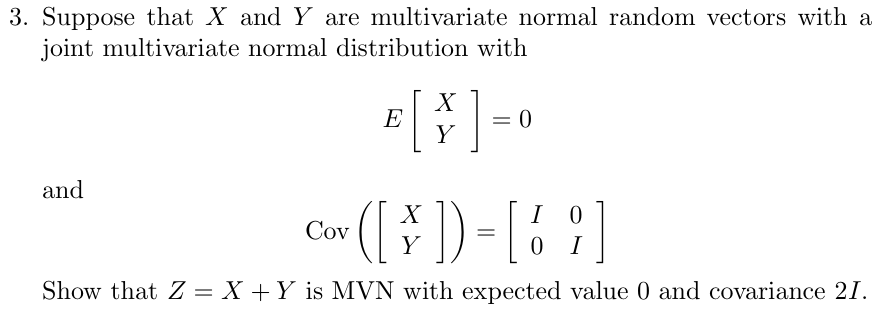
\includegraphics[width=0.8\textwidth]{./images/prob3_statement.png}
\end{figure}

\subsection*{Solution}

Given the problem statement, let random vectors $\bv{X}$ and $\bv{Y}$ be of equal dimension such that

\begin{align*}
	\bv{X},\,\bv{Y} \sim \textrm{N}\left(0,\,I\right)
\end{align*}

Creating a new random vector $\bv{Z} = \bv{X} + \bv{Y}$, the expected value of $\bv{Z}$ is

\begin{align*}
	\E{\bv{Z}} &= \E{\bv{X} + \bv{Y}} \\
	\\
	&= \E{\bv{X}} + \E{\bv{Y}} \\
	\\
	&= \bv{0} + \bv{0} \\
	\\
	&= \bv{0} \,\,\,\,\, \textcolor{green}{\checkmark}
\end{align*}

To determine the covariance of $\bv{Z}$, we must first find a matrix $A$ such that $\bv{Z} = \bv{X} + \bv{Y}$. $A$ is defined as:

\begin{align*}
	\bv{Z} &= A \begin{bmatrix} \bv{X} \\ \bv{Y} \end{bmatrix}
	\\
	\bv{Z} &= \begin{bmatrix} I & I \end{bmatrix} \begin{bmatrix} \bv{X} \\ \bv{Y} \end{bmatrix}
	\\
	\\
	\\
	A &\defeq \begin{bmatrix} I & I \end{bmatrix}
\end{align*}

The covariance of $\bv{Z}$ is given by the transformation $\bv{Z} = A C A^T$, which is shown below.

\begin{align*}
	\Cov{\bv{Z}} &= A \Cov{\begin{bmatrix} \bv{X} \\ \bv{Y} \end{bmatrix}} A^T \\
	\\
	&= \begin{bmatrix} I & I \end{bmatrix} \begin{bmatrix} I & 0 \\ 0 & I \end{bmatrix} \begin{bmatrix} I \\ I \end{bmatrix} \\
	\\
	&= \begin{bmatrix} I & I \end{bmatrix} \begin{bmatrix} I \\ I \end{bmatrix} \\
	\\
	&= I + I \\
	\\
	&= 2I \,\,\,\,\, \textcolor{green}{\checkmark}
\end{align*}